\documentclass[dvips, lscape, 6pt]{beamer}

%%%%%%%%%%%%%%%%%%%%%%%%%%%%%%%%%%%%%%%%%%%%%%%%%%%%%%%%%%%%%%%%%%%%%%
% Maths
\usepackage{amsfonts, amsmath, amssymb}
\newcommand{\coefbin}[2]{\left(
    \begin{array}{c} #1 \\ #2 \end{array}
  \right)}
\newcommand{\bbullet}{\bullet\bullet}
\newcommand{\bbbullet}{\bbullet\bullet}
\newcommand{\bbbbullet}{\bbbullet\bullet}
\newcommand{\Bcal}{\mathcal{B}}
\newcommand{\Ccal}{\mathcal{C}}
\newcommand{\Dcal}{\mathcal{D}}
\newcommand{\Ecal}{\mathcal{E}}
\newcommand{\Gcal}{\mathcal{G}}
\newcommand{\Mcal}{\mathcal{M}}
\newcommand{\Ncal}{\mathcal{N}}
\newcommand{\Pcal}{\mathcal{P}}
\newcommand{\Qcal}{\mathcal{Q}}
\newcommand{\Rcal}{\mathcal{R}}
\newcommand{\Hcal}{\mathcal{H}}
\newcommand{\Jcal}{\mathcal{J}}
\newcommand{\Lcal}{\mathcal{L}}
\newcommand{\Tcal}{\mathcal{T}}
\newcommand{\Ucal}{\mathcal{U}}
\newcommand{\Xcal}{\mathcal{X}}
\newcommand{\Zcal}{\mathcal{Z}}
\newcommand{\etabar}{\overline{\eta}}
\newcommand{\pibar}{\overline{\pi}}
\newcommand{\alphabf}{\mbox{\mathversion{bold}{$\alpha$}}}
\newcommand{\betabf}{\mbox{\mathversion{bold}{$\beta$}}}
\newcommand{\gammabf}{\mbox{\mathversion{bold}{$\gamma$}}}
\newcommand{\mubf}{\mbox{\mathversion{bold}{$\mu$}}}
\newcommand{\pibf}{\mbox{\mathversion{bold}{$\pi$}}}
\newcommand{\Pibf}{\mbox{\mathversion{bold}{$\Pi$}}}
\newcommand{\psibf}{\mbox{\mathversion{bold}{$\psi$}}}
\newcommand{\Sigmabf}{\mbox{\mathversion{bold}{$\Sigma$}}}
\newcommand{\taubf}{\mbox{\mathversion{bold}{$\tau$}}}
\newcommand{\thetabf}{\mbox{\mathversion{bold}{$\theta$}}}
\newcommand{\Abf}{{\bf A}}
\newcommand{\Ebf}{{\bf E}}
\newcommand{\Hbf}{{\bf H}}
\newcommand{\Ibf}{{\bf I}}
\newcommand{\Obf}{{\bf 0}}
\newcommand{\Sbf}{{\bf S}}
\newcommand{\mbf}{{\bf m}}
\newcommand{\ubf}{{\bf u}}
\newcommand{\vbf}{{\bf v}}
\newcommand{\xbf}{{\bf x}}
\newcommand{\Xbf}{{\bf X}}
\newcommand{\ybf}{{\bf y}}
\newcommand{\Zbf}{{\bf Z}}
\newcommand{\Esp}{{\mathbb E}}
\newcommand{\Corr}{{\mathbb C}\mbox{orr}}
\newcommand{\Nbb}{\mathbb{N}}
\newcommand{\Nm}{N(\mbf)}
\newcommand{\mum}{\mu(\mbf)}
\newcommand{\obs}{\text{obs}}
\newcommand{\ERMG}{\text{EMRG}}
\newcommand{\Ibb}{{\mathbb I}}
\newcommand{\Omegas}{\underset{s}{\Omega}}
\newcommand{\Var}{{\mathbb V}}
\newcommand{\Pro}{\mathbb{P}}
\newcommand{\Rbb}{\mathbb{R}}
\newcommand{\RX}{R_{\Xbf}}
\newcommand{\Vsf}{\mathsf{V}}
\newcommand{\Starsf}{\mathsf{*}}

%%%%%%%%%%%%%%%%%%%%%%%%%%%%%%%%%%%%%%%%%%%%%%%%%%%%%%%%%%%%%%%%%%%%%%
% Couleur et graphiques
% \usepackage{color}
\usepackage{graphics}
\usepackage{epsfig}
% \usepackage{pstcol}

%%%%%%%%%%%%%%%%%%%%%%%%%%%%%%%%%%%%%%%%%%%%%%%%%%%%%%%%%%%%%%%%%%%%%%
% Texte
\usepackage[english]{babel}
\usepackage[latin1]{inputenc}
\usepackage{times}
\usepackage[T1]{fontenc}
\usepackage{url}
\newcommand{\refer}[1]{\textcolor{green}{\sl #1}}
\newcommand{\emphase}[1]{\textcolor{blue}{\sl #1}}

%%%%%%%%%%%%%%%%%%%%%%%%%%%%%%%%%%%%%%%%%%%%%%%%%%%%%%%%%%%%%%%%%%%%%%
% Beamer
\usepackage{beamerthemesplit}
\usetheme{Darmstadt}
% \usefonttheme[onlylarge]{structurebold}
\setbeamerfont*{frametitle}{size=\normalsize,series=\bfseries}
\setbeamertemplate{navigation symbols}{}

%%%%%%%%%%%%%%%%%%%%%%%%%%%%%%%%%%%%%%%%%%%%%%%%%%%%%%%%%%%%%%%%%%%%%%
% En-t�te
\title[Latent structure in graphs]
{
  Uncovering latent structure in valued graphs:
  A variational approach
}

\author[Mariadassou, Robin]
{
  M. Mariadassou \and \underline{S. Robin}\inst{1}
}

\institute[AgroParisTech/INRA]
{
  UMR 518 AgroPairsTech / INRA Applied Mathematics \& Computer Sciences:

  {\tt www.agroparistech.fr/stat-genome/}

  Statistics for Systems Biology group: {\tt genome.jouy.inra.fr/ssb/}
}

\date{\today}

\setcounter{tocdepth}{1}

%%%%%%%%%%%%%%%%%%%%%%%%%%%%%%%%%%%%%%%%%%%%%%%%%%%%%%%%%%%%%%%%%%%%%%
%%%%%%%%%%%%%%%%%%%%%%%%%%%%%%%%%%%%%%%%%%%%%%%%%%%%%%%%%%%%%%%%%%%%%%
\begin{document}
%%%%%%%%%%%%%%%%%%%%%%%%%%%%%%%%%%%%%%%%%%%%%%%%%%%%%%%%%%%%%%%%%%%%%%
%%%%%%%%%%%%%%%%%%%%%%%%%%%%%%%%%%%%%%%%%%%%%%%%%%%%%%%%%%%%%%%%%%%%%%

%%%%%%%%%%%%%%%%%%%%%%%%%%%%%%%%%%%%%%%%%%%%%%%%%%%%%%%%%%%%%%%%%%%%%%%%
\begin{frame}

  \titlepage
%   {\bf Research report:}
%   \url{genome.jouy.inra.fr/ssb/preprint/SSB-RR-10.valued-graphs.pdf}

\end{frame}

%%%%%%%%%%%%%%%%%%%%%%%%%%%%%%%%%%%%%%%%%%%%%%%%%%%%%%%%%%%%%%%%%%%%%%%%
\begin{frame}{Outline}

  \tableofcontents

\end{frame}

%%%%%%%%%%%%%%%%%%%%%%%%%%%%%%%%%%%%%%%%%%%%%%%%%%%%%%%%%%%%%%%%%%%%%
%%%%%%%%%%%%%%%%%%%%%%%%%%%%%%%%%%%%%%%%%%%%%%%%%%%%%%%%%%%%%%%%%%%%%
\section{Looking for structure in networks}

\begin{frame}
  \noindent
  \begin{tabular}{cc}
    \begin{tabular}{p{5cm}}
      Networks \dots
      \begin{itemize}
      \item<1-> Arise in many fields:
        \begin{itemize}
        \item[\bf{$\rightarrow$}] Biology, Chemistry
        \item[\bf{$\rightarrow$}] Physics, Internet.
        \end{itemize}
      \item<1-> Represent an interaction pattern:
        \begin{itemize}
        \item[\bf{$\rightarrow$}] $\mathcal{O}(n^2)$ interactions
        \item[\bf{$\rightarrow$}] between $n$ elements.
        \end{itemize}
      \item<1-> Have a topology which:
        \begin{itemize}
        \item[\bf{$\rightarrow$}] reflects the structure / function
          relationship
        \end{itemize}
      \end{itemize}
    \end{tabular}
    &
    \begin{tabular}{c}
      \psfig{file=../Figures/caida2_lg(brown).ps, angle=270, width=5cm} \\
      \begin{tiny} From Barab\'asi website \end{tiny}
    \end{tabular}
  \end{tabular}
\end{frame}

%%%%%%%%%%%%%%%%%%%%%%%%%%%%%%%%%%%%%%%%%%%%%%%%%%%%%%%%%%%%%%%%%%%%%
\begin{frame}
  {Uncovering structure: A simple example}
  \vspace{-1cm}
  $$
  \begin{tabular}{c}
    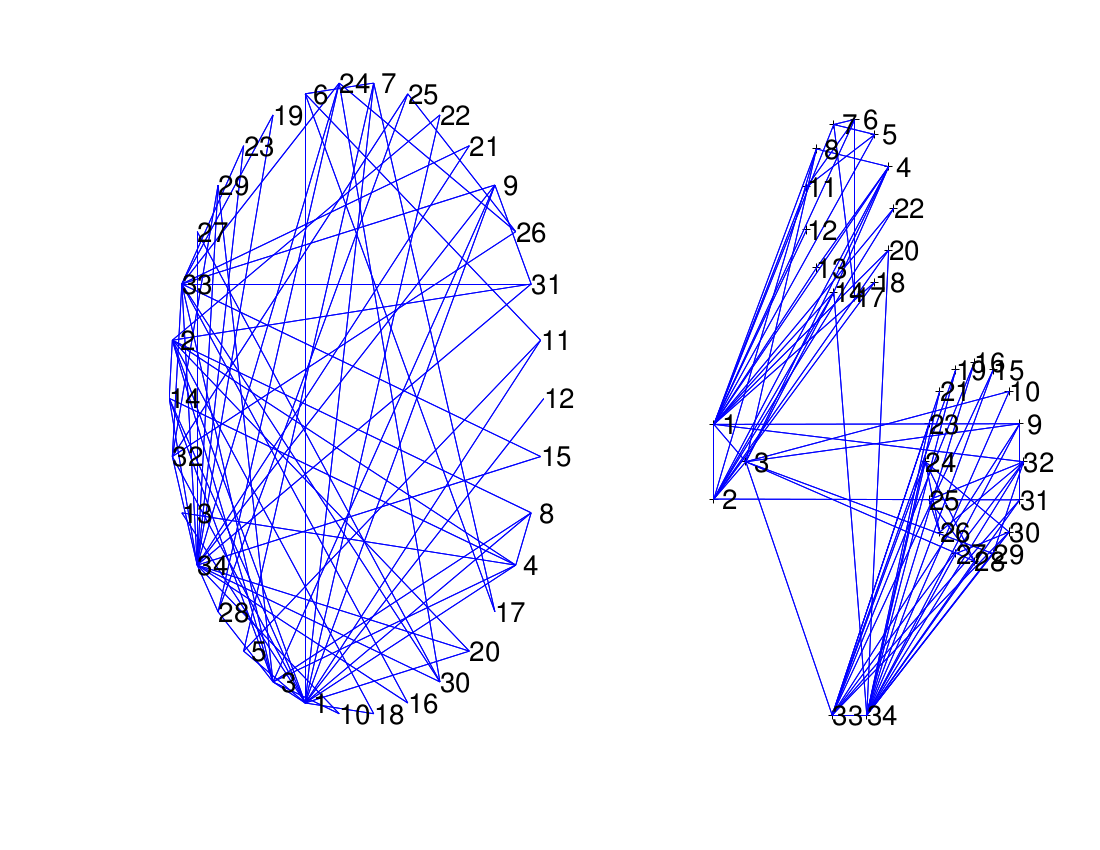
\epsfig{file = ../Figures/Karate-Graph.eps, clip=, width=3.5cm,
      height=10cm, angle=270}
    \\
    \epsfig{file = ../Figures/Karate-Dotplot.eps, clip=, width=3.5cm,
      height=10cm, angle=270}
  \end{tabular}
  $$
\end{frame}

%%%%%%%%%%%%%%%%%%%%%%%%%%%%%%%%%%%%%%%%%%%%%%%%%%%%%%%%%%%%%%%%%%%%
\subsection{Heterogeneity in random graphs}

\begin{frame}

  Nodes may have different connectivity behaviour.

  {\bf Looking for connected sub-groups:}
  \begin{itemize}
  \item<1-> Detection of cliques or groups of highly
    connected nodes: \refer{Gethor \& Diehl, 04}
  \item<1-> Edge betweenness: \refer{Girvan \& Newman, 02}
  \item<1-> Spectral clustering: \refer{Von Luxburg \& al.,
      07}
  \end{itemize}

  {\bf Model based:}
  \begin{itemize}
  \item<1-> Underlying topology: \refer{Hoff \& al., 02}
    (Latent space)
  \item<1-> Mixture model \refer{Nowicki \& Snijders, 01}
    (Block structure), \refer{Daudin \& al., 08} (Mixture for graphs)
  \item<1-> General model for heterogeneous networks:
    \refer{Bollob\'as \ al., 07} (Topolical properties: Giant component,
    diameter, degree distribution = compound Poisson, {\it etc.}).
  \item<1-> General review on random graph models:
    \refer{Pattison \& Robbins, 07}
  \end{itemize}
\end{frame}

%%%%%%%%%%%%%%%%%%%%%%%%%%%%%%%%%%%%%%%%%%%%%%%%%%%%%%%%%%%%%%%%%%%%
\subsection{Inhomogeneous random graphs}

\begin{frame}
  {\bf General definition for binary graphs.} (\refer{Bollob\'as \ al., 07})
  \begin{itemize}
  \item<1-> $n$ nodes $(i = 1 \dots n$)
  \item<1-> $n(n-1)/2$ possible edges: $X_{ij} = \Ibb\{ i \sim j\}$
  \item<1-> Each $i$ is characterised by a \emphase{latent
      variable} $Z_i$ sampled in some space $\Zcal$ with distribution
    $\alpha$:
    $$
    \{Z_i\}_i \mbox{ i.i.d.}, \qquad Z_i \sim \alpha
    $$
  \item<1-> Edge $(i, j)$ is present with probability
    $\pi(Z_i, Z_j)$, where $\pi$ is a \emphase{kernel function}:
    $$
    \{X_{ij}\}_{i, j} \mbox{ independent given } \{Z_i\}_i, \qquad X_{ij}
    \sim \Bcal[\pi(Z_i, Z_j)].
    $$
  \end{itemize}
  {\bf Latent space:}
  $\displaystyle{
    \Zcal = \Rbb^k, \qquad \pi(z, z') = \frac{\exp(a - |z-z'|)}{1 + \exp(a
      - |z-z'|)}.
    }$

  {\bf Mixture model:}
  $\displaystyle{
    \Zcal = \{1, \dots, Q\}, \qquad \pi(z, z') = \pi_{q\ell} \mbox{ for } z
    = q, z' = \ell.
    }$
\end{frame}

%%%%%%%%%%%%%%%%%%%%%%%%%%%%%%%%%%%%%%%%%%%%%%%%%%%%%%%%%%%%%%%%%%%%%
%%%%%%%%%%%%%%%%%%%%%%%%%%%%%%%%%%%%%%%%%%%%%%%%%%%%%%%%%%%%%%%%%%%%%
\section{Mixture model for valued graphs}

\begin{frame}
  {\bf Our approach}
  \begin{itemize}
  \item<1-> is model based:
    $$
    \mbox{Mixture model}
    $$
  \item<1-> deals with valued graphs:
    $$
    \mbox{$X_{ij} \in \{0, 1\}, \Nbb, \Rbb, \Rbb^d, {\it etc.}$}
    $$
  \item<1-> and makes frequentist inference using a
    variational method :
    $$
    \mbox{Approximate maximum likelihood.}
    $$
  \end{itemize}
\end{frame}

%%%%%%%%%%%%%%%%%%%%%%%%%%%%%%%%%%%%%%%%%%%%%%%%%%%%%%%%%%%%%%%%%%%%%
\subsection{Model}

\begin{frame}
  \begin{itemize}
  \item<1-> $n$ nodes $(i = 1 \dots n$);
  \item<1-> each node $i$ belong to class $q$ with
    probability $\alpha_q$:
    $$
    \{Z_i\}_i \mbox{ i.i.d.}, \qquad Z_i \sim \Mcal(1; \alphabf)
    $$
    where $\alphabf = (\alpha_1, \dots \alpha_Q)$;
  \item<1-> The values of the edges $\{X_{ij}\}_{i,
      j}$ are conditionally independent given the $Z_i$'s:
    $$
    (X_{ij} \;|\; Z_i = q, Z_j = \ell) \sim f_{q\ell}(\cdot).
    $$
    where $f_{q\ell}(\cdot)$ is some parametric distribution
    $f_{q\ell}(x) = f(x; \theta_{q\ell})$. \\ ~\\
  \end{itemize}
  We denote: $\Zbf = \{Z_i\}_i$, $\Xbf = \{X_{ij}\}_{i, j}$, $\thetabf =
  \{\theta_{q\ell}\}_{q, \ell}$, $\gammabf = (\alphabf, \thetabf)$.
\end{frame}

%%%%%%%%%%%%%%%%%%%%%%%%%%%%%%%%%%%%%%%%%%%%%%%%%%%%%%%%%%%%%%%%%%%%%
\subsection{Some distributions $f_{q\ell}$}

\begin{frame}

  {\bf Bernoulli $\Bcal(\pi_{ql})$.} Binary oriented or
  non-oriented \emphase{interaction graphs}: \\
  Relation network, protein-protein interaction, gene regulation.

  {\bf Multinomial $\Mcal(\pibf_{ql})$.} \emphase{Labelled edges}: \\
  Social networks ('friend', 'lover', colleague'), Directed graphs with
  correlated edges (' ', '$\rightarrow$', '$\leftarrow$',
  '$\leftrightarrow$').

  {\bf Poisson $\Pcal(\lambda_{ql})$.} The edge value is a \emphase{count}:
  \\
  Number of co-publications of two authors, Number of times two species
  were observed in the same place, Number of alleles shared by two
  species.

  {\bf Gaussian $\Ncal(\mu_{q\ell}, \sigma^2)$.} \emphase{Traffic
    intensity}: \\
  Airport network, Electric network.

  {\bf Linear regression.} If \emphase{covariates} $\ybf_{ij}$ are
  available for each couple of nodes:
  $$
  X_{ij} = \ybf_{ij} \betabf_{q\ell} + E_{ij}, \qquad \{E_{ij}\}_{i, j}
  \mbox{ independent, } E_{ij} \sim \Ncal(0, \sigma^2).
  $$
\end{frame}

%%%%%%%%%%%%%%%%%%%%%%%%%%%%%%%%%%%%%%%%%%%%%%%%%%%%%%%%%%%%%%%%%%%%%
%%%%%%%%%%%%%%%%%%%%%%%%%%%%%%%%%%%%%%%%%%%%%%%%%%%%%%%%%%%%%%%%%%%%%
\section{Variational inference}

\subsection{Maximum Likelihood Inference}

\begin{frame}
  {\bf Likelihoods.} The log-likelihood of the complete dataset
  ($\Xbf, \Zbf$) is
  \begin{eqnarray*}
    \log{\Pro(\Zbf,\Xbf; \alphabf, \thetabf)} & = & \log\Pro(\Zbf; \alphabf) +
    \log{\Pro(\Xbf | \Zbf; \thetabf)} \\
    & = & \sum_i \sum_q Z_{iq}\log{\alpha_q} + \sum_{i \neq j}
    \sum_{q,\ell} Z_{iq}Z_{j\ell}\log{f_{q\ell}(X_{ij})}.
  \end{eqnarray*}
  The log-likelihood of the observed dataset ($\Xbf$) is
  $$
  \log{\Pro(\Xbf; \alphabf, \thetabf)} = \sum_{\Zbf} \log{\Pro(\Zbf,\Xbf;
    \alphabf, \thetabf)}
  $$
  and cannot be evaluated since $\Zbf$ may take $Q^n$ different
  values. \\

  {\bf Most popular solution:} E-M algorithm.
\end{frame}

%%%%%%%%%%%%%%%%%%%%%%%%%%%%%%%%%%%%%%%%%%%%%%%%%%%%%%%%%%%%%%%%%%%%%
\begin{frame}
  {\bf E-M algorithm.} To achieve the E-step, we need to calculate
  the conditional distribution of the unobserved data given the observed
  ones: $\log{\Pro(\Zbf|\Xbf)}$.

  {\bf Due to intricate dependencies} this distribution is
  \emphase{intractable}:
  $$
  \begin{tabular}{p{11cm}p{11cm}}
    {\bf Dependency graph} (oriented) & {\bf Moral graph}
    (parents are married) \\
    \\
    Edge $X_{ij}$ only depends on its two parents $Z_1$ and $Z_2$
    &
    Conditional on the edges, labels $Z_i$'s all depend on each others \\
                                %\\
    \hspace{-1cm}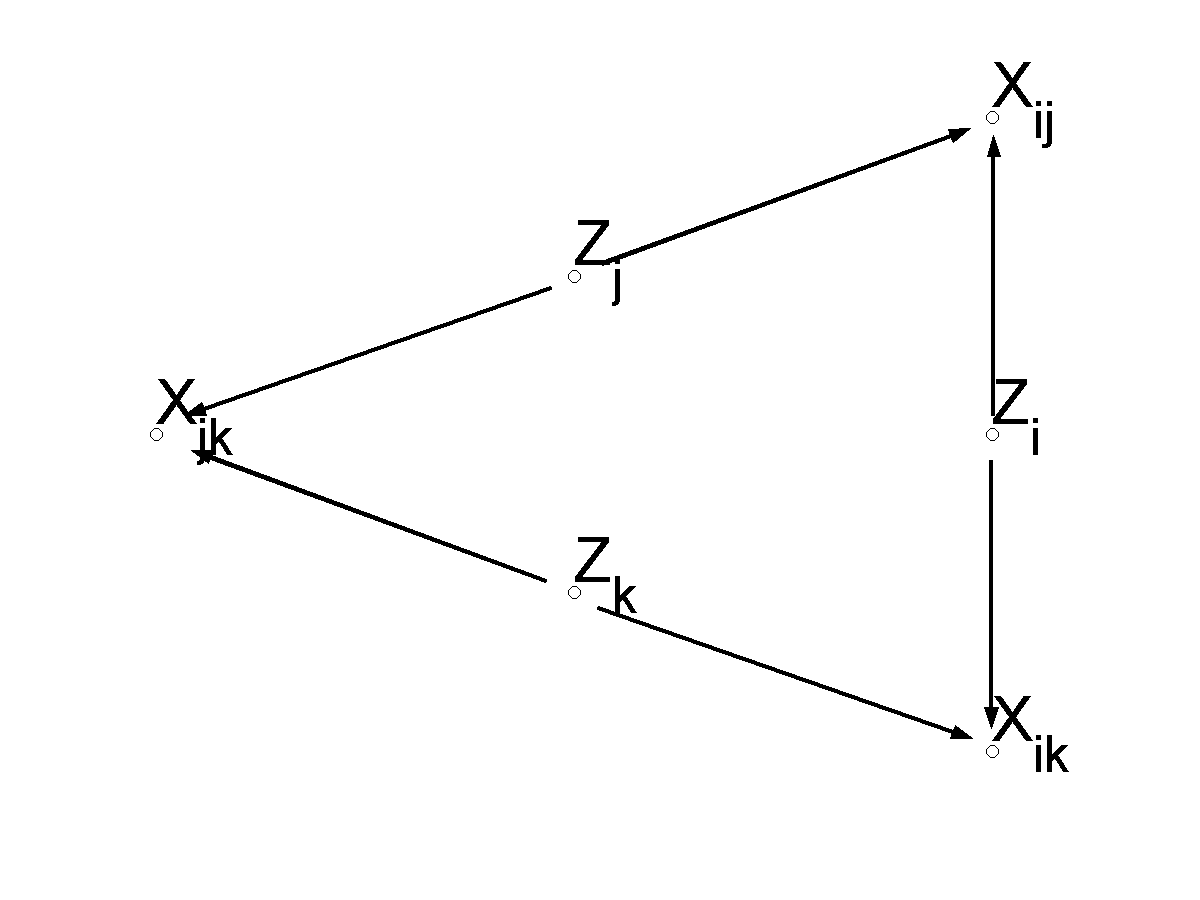
\epsfig{file = ../figures/FigNetworks-DepGraph.eps, clip=,
      angle=270, width=11cm}
    &
    \hspace{-1cm}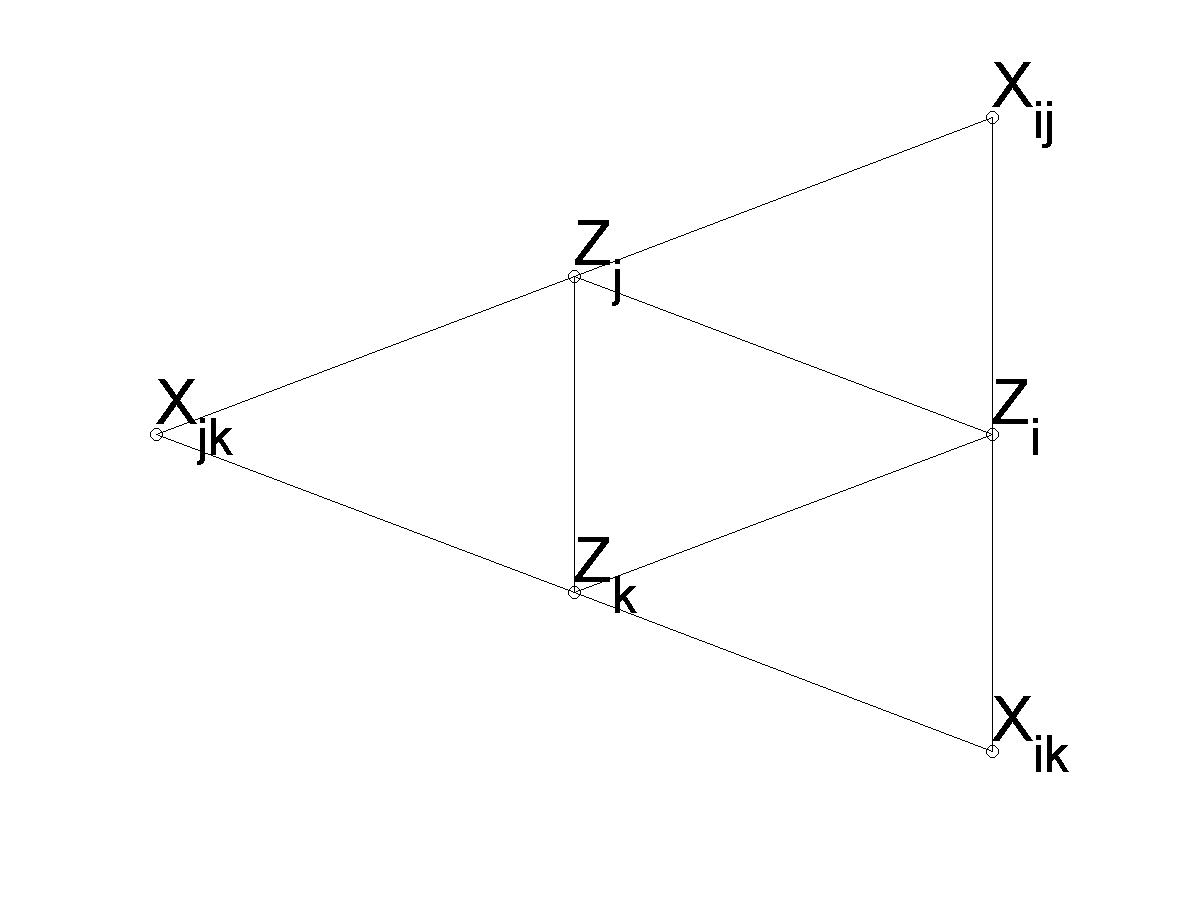
\epsfig{file =
      ../figures/FigNetworks-DepGraph-Moral.eps, clip=, angle=270,
      width=11cm} \\
    \multicolumn{2}{c}{\vspace{-0.5cm}$\Rightarrow$ All edges are
      actually \emphase{'neighbours'} (unlike for Bayesian networks).}
  \end{tabular}
  $$
\end{frame}

%%%%%%%%%%%%%%%%%%%%%%%%%%%%%%%%%%%%%%%%%%%%%%%%%%%%%%%%%%%%%%%%%%%%%
\subsection{Variational strategy}

\begin{frame}
  {\bf Choice of $\RX$.} $\RX$ approximates the conditional
  distribution $\Pro(\Zbf|\Xbf)$. We want it to be
  \begin{itemize}
  \item<1-> tractable (e.g. factorised):
    $$
    \RX(\Zbf) = \prod_i h(\Zbf_i, \taubf_i)
    $$
    where $h(\cdot, \taubf)$ denotes the multinomial distribution;
  \item<1-> as close to $\Pro(\Zbf|\Xbf)$ as possible:
    $$
    \widehat{\taubf} = \arg \min
    KL[\RX(\cdot),\Pro(\cdot|\Xbf;\alphabf, \thetabf)].
    $$
  \end{itemize}
  We get
  $$
  \Jcal(\RX,\alphabf, \thetabf) = - \sum_i \sum_q \tau_{iq} \log{\tau_{iq}} +
  \sum_i \sum_q \tau_{iq} \log{\alpha_q} + \sum_{i \neq j} \sum_{q,\ell}
  \tau_{iq} \tau_{j\ell} \log{f_{q\ell}(X_{ij})}.
  $$
  The $\tau_i$'s are interpreted as \emphase{approximate posterior
    probabilities $\Pro\{Z_i = q | \Xbf\}$};
\end{frame}

%%%%%%%%%%%%%%%%%%%%%%%%%%%%%%%%%%%%%%%%%%%%%%%%%%%%%%%%%%%%%%%%%%%%%
\subsection{Estimation algorithm}

\begin{frame}
  The optimisation of $\Jcal(\RX,\alphabf, \thetabf)$ is achieved via two
  alternative steps.

  {\bf M-step:} Maximises $\Jcal(\RX,\alphabf, \thetabf)$ w.r.t. $\alphabf, \thetabf =
  (\alphabf, \thetabf)$ given $\taubf$. We get
  $$
  \widehat{\alpha}_q = \frac1n \sum_i \tau_{iq}, \qquad
  \widehat{\theta}_{q\ell} = \arg\underset{\theta_{q\ell}}{\max} \sum_{i
    \neq j} \tau_{iq}\tau_{j\ell}\log{f(X_{ij}; \theta_{q\ell})}.
  $$

  {\bf Fix point relation.} Find the optimal $\taubf$ given
  $(\alphabf, \thetabf)$. We end up with a fix point relation.
  \begin{itemize}
  \item<1-> Oriented graphs:
    $$
    \log \widehat{\tau}_{iq} = \mbox{cst} + \log \alpha_q + \sum_{j
      \neq i} \sum_{\ell} \widehat{\tau}_{j\ell} \left[\log
      f(X_{ij}; \theta_{q\ell}) \log f(X_{ji}; \theta_{\ell q})\right].
    $$
  \item<1-> Non-oriented graphs:
    $$
    \log \widehat{\tau}_{iq} = \mbox{cst} + \log \alpha_q + \sum_{j
      \neq i} \sum_{\ell} \widehat{\tau}_{j\ell} \log f(X_{ij};
    \theta_{q\ell}).
    $$
  \end{itemize}

\end{frame}

%%%%%%%%%%%%%%%%%%%%%%%%%%%%%%%%%%%%%%%%%%%%%%%%%%%%%%%%%%%%%%%%%%%%%
\subsection{Model selection}

\begin{frame}
  {\bf Penalised likelihood.} Standard criteria, such as BIC or
  AIC are based on the log-likelihood of observed data $\log
  \Pro(\Xbf)$, so they can not be used here.

  {\bf Integrated Classification Likelihood (ICL).} The ICL
  criterion (\refer{Biernacki \& al., 00}) is an approximation of the
  complete-data integrated log-likelihood:
  $$
  \log \Pro(\Xbf, \Zbf| m_Q) = \int \log \Pro(\Xbf, \Zbf |
  \gammabf,m_Q) g(\gammabf|m_Q) d\gammabf,
  $$
  where $\log \Pro(\Xbf, \Zbf | \gammabf,m_Q)$ is the log-likelihood
  of model $m_Q$ with $Q$ classes.

  We get
  $$
  ICL(m_Q) = \underset{\gammabf}{\max} \log \Pro(\Xbf,
  \widehat{\Zbf} |\gammabf, m_Q) - \frac{1}{2} \left\{ P_Q \log
    [n(n-1)] - (Q-1) \log(n) \right\}.
  $$
  where $P_Q$ denotes the number of parameters in $\thetabf$ and
  $\widehat{\Zbf}$ can be replaced by $\widehat{\taubf}$ or by the
  Maximum A posteriori (MAP) prediction of $\Zbf$.
\end{frame}

%%%%%%%%%%%%%%%%%%%%%%%%%%%%%%%%%%%%%%%%%%%%%%%%%%%%%%%%%%%%%%%%%%%%%
\section{Applications}

\subsection{Metabolic network of {\sl E. coli}}

\begin{frame}
  {\bf Dataset.}
  \begin{itemize}
  \item<1-> The network is made of 605 reaction (nodes) and
    1782 edges (\refer{V Lacroix \& M.-F. Sagot, INRIA}).
  \item<1-> Reactions $i$ and $j$ are connected if the
    compound of $i$ is the substrate of $j$.
  \item<1-> Because most reactions are reversible, the
    network is not oriented.
  \item<1-> The only information about edges is terms of
    presence/absence.
  \end{itemize}
  {\bf Results}
  \begin{itemize}
  \item<1-> The ICL criterion applied to a mixture with
    Bernoulli edge values select $\widehat{Q} = 21$ classes.
  \item<1-> Groups 1 to 20 gather reactions involving
    all the \emphase{same compound} either as a substrate or as a
    product.
  \item<1-> A compound (chorismate, pyruvate,
    ATP,\emph{etc}) can be associated to each group.
  \end{itemize}
\end{frame}


%%%%%%%%%%%%%%%%-------------------------%%%%%%%%%%%%%%%%%%%%%%%%%%%%
%%%%%%%%%%%%%%%%-------------------------%%%%%%%%%%%%%%%%%%%%%%%%%%%%
\end{document}
%%%%%%%%%%%%%%%%-------------------------%%%%%%%%%%%%%%%%%%%%%%%%%%%%
%%%%%%%%%%%%%%%%-------------------------%%%%%%%%%%%%%%%%%%%%%%%%%%%%


%%%%%%%%%%%%%%%%%%%%%%%%%%%%%%%%%%%%%%%%%%%%%%%%%%%%%%%%%%%%%%%%%%%%%
\begin{frame}
  {\bf Dot-plot representation.} \\
  \begin{tabular}{cc}
    \begin{tabular}{p{12cm}}
      \begin{itemize}
      \item<1-> Classes 1 and 16 constitute a \emphase{single clique}
        corresponding to a single compound (pyruvate),
      \item<1-> They are split into two classes because they
        \emphase{interact differently with classes 7} (CO2) and 10
        (AcetylCoA)
      \item<1-> Connectivity matrix (sample):
        $$
        \begin{array}{c|cccc}
          q, \ell & 1 & 7 & 10 & 16 \\
          \hline
          1  & \textcolor{red}{1.0} & & & \\
          7  & \textcolor{green}{.11} & .65 & &  \\
          10 & \textcolor{green}{.43} & & .67 & \\
          16 & \textcolor{red}{1.0} & \textcolor{yellow}{.01} &
          \textcolor{yellow}{\epsilon} & \textcolor{red}{1.0}
        \end{array}
        $$
      \end{itemize}
    \end{tabular}
    &
    \begin{tabular}{c}
      \epsfig{file = ../Figures/Ecoli-Complet-ERMG-Ward-Q21_class3.ps,
        height=12cm, width=12cm, clip=, angle=90, bbllx=33, bblly=64,
        bburx=565, bbury=389} \\
      Adjacency matrix \\
      (zoom on the 20 first classe)
    \end{tabular}
  \end{tabular}
\end{frame}

%%%%%%%%%%%%%%%%%%%%%%%%%%%%%%%%%%%%%%%%%%%%%%%%%%%%%%%%%%%%%%%%%%%%%
\subsection{Gene regulations in {\sl A. Thaliana}}

\begin{frame}
  {\bf Dataset.} \emphase{Partial correlations} between the expression
  levels of 800 genes in various conditions (\refer{Opgen-Rhein \&
    Strimmer, 06}). \\
  ~\\
  \begin{tabular}{cc}
    \hspace{-1cm}
    \begin{tabular}{p{12cm}}
      {\bf Dot-plot.} Dot size = absolute correlation, Color =
      sign (\textcolor{red}{$-$}, {$+$}). \\
      ~\\
      {\bf Results.}
      \begin{itemize}
      \item<1-> Using a Gaussian model, we get $\widehat{Q}
        = 7$ classes.
      \item<1-> Groups are made of positively correlated
        genes.
      \item<1-> Between group correlations are weaker than
        within-group correlation and have different signs (see classes
        3/4 with class 7).
      \item<1-> Total computational time for $Q=1..15$
        classes on a standard PC: 1h.
      \end{itemize}
    \end{tabular}
    &
    \begin{tabular}{c}
      \hspace{-1cm}
      \epsfig{file = ../Figures/GauHo_Q7_dotplot.eps, width=13cm,
        height=13cm, clip=}
    \end{tabular}
  \end{tabular}
\end{frame}

%%%%%%%%%%%%%%%%%%%%%%%%%%%%%%%%%%%%%%%%%%%%%%%%%%%%%%%%%%%%%%%%%%%%%
\subsection{Fungus - Tree interactions}

\begin{frame}
  {\bf Dataset.} Interactions between 154 fungi and 51
  trees European species. Fungus $f$ is connected to tree $t$ if it has
  been collected on it (\refer{Data from C. Vacher, INRA}).

  {\bf Projected graphs.} For each species we define the projected
  graph:
  $$
  \begin{array}{lrcl}
    \mbox{for trees} \quad & X_{tt'} & = & \mbox{Number of common
      fungi,} \\
    \\
    \mbox{for fungi} \quad & X_{ff'} & = & \mbox{Number of common trees.}
  \end{array}
  $$

  {\bf Poisson model.} For both species, we assume that the
  intensities have Poisson distributions: $X
  \sim\Pcal(\lambda_{q\ell})$.

  {\bf Number of classes.} The ICL criterion selects
  \begin{itemize}
  \item<1-> 5 classes for trees
  \item<1-> and 6 classes for fungi.
  \end{itemize}
\end{frame}

%%%%%%%%%%%%%%%%%%%%%%%%%%%%%%%%%%%%%%%%%%%%%%%%%%%%%%%%%%%%%%%%%%%%%
\begin{frame}
  \noindent
  \begin{tabular}{cc}
    \begin{tabular}{p{11cm}}
      \subsection{Fungus network}
      \\
      \epsfig{file = ../Figures/Fungus_Poiss_Q6_dotplot.eps,
        width=12cm, height=12cm, clip=} \\
      \begin{itemize}
      \item<1-> A group of generalist fungi is detected.
      \item<1-> Others are more specific.
      \end{itemize}
    \end{tabular}
    &
    \begin{tabular}{p{11cm}}
      \subsection{Tree network}
      \\
      \epsfig{file = ../Figures/Tree_Poiss_Q5_dotplot.eps,
        width=8cm, height=8cm, clip=}
      \\
      \begin{itemize}
      \item<1-> Trees are mainly clustered according to
        the number of fungi they host.
      \item<1-> Tree groups are less contrasted.
      \end{itemize}
      \\ \\ \\ \\
    \end{tabular}
  \end{tabular}
\end{frame}

%%%%%%%%%%%%%%%%%%%%%%%%%%%%%%%%%%%%%%%%%%%%%%%%%%%%%%%%%%%%%%%%%%%%%
\subsection{Crossed clusterings}

\begin{frame}
  \noindent
  \begin{tabular}{cc}
    \begin{tabular}{p{16cm}}
      The comparison of the two clusterings exhibits \emphase{specific
        correspondences} between groups of fungi (rows) and trees (columns). \\
      \\ \\
      {\bf Work in progress.} Compare these groups according to
      their phyla, the time of their introduction in Europe, {\it
        etc.}. \\
      \\ \\
      {\bf Biclustering.} A direct clustering could be performed
      on the interaction matrix Fungi $\times$ Tree. The method
      proposed by \refer{Govaert \& Nadif (05)} also relies on a
      variational approach. \\ \\
    \end{tabular}
    &
    \begin{tabular}{p{10cm}}
      \epsfig{file = ../Figures/CompCluster_QF6_QT5.eps,
        width=7cm, height=15cm, clip=}
    \end{tabular}
  \end{tabular}
\end{frame}

%%%%%%%%%%%%%%%%%%%%%%%%%%%%%%%%%%%%%%%%%%%%%%%%%%%%%%%%%%%%%%%%%%%%%
%%%%%%%%%%%%%%%%%%%%%%%%%%%%%%%%%%%%%%%%%%%%%%%%%%%%%%%%%%%%%%%%%%%%%
\section{Discussion}

\subsection{Inference for heterogeneous valued graphs}

\begin{frame}
  \begin{itemize}
  \item<1-> Mixture models constitutes a natural way to
    describe heterogeneity in a network.
  \item<1-> The variational approach is a general and
    efficient alternative to MCMC algorithms.
  \end{itemize}
\end{frame}

%%%%%%%%%%%%%%%%%%%%%%%%%%%%%%%%%%%%%%%%%%%%%%%%%%%%%%%%%%%%%%%%%%%%%
\subsection{Simulation of 'realistic' networks}

\begin{frame}
  \begin{itemize}
  \item<1-> 'Realistic' heterogeneous networks can be
    simulated according to mixture models with given parameters.
  \item<1-> The \emphase{Expected Degree Distribution (EDD)}
    model (\refer{Park \& Newman, 03}, \refer{Chung \& Lu, 02}) is
    another special case of heterogeneous binary network:
    \begin{itemize}
    \item<1-> For each node $i$, draw its \emphase{expected degree $D_i$} in
      the empirical degree distribution $F$ of a given network.
                                %: $\{D_i\} \mbox{ i.i.d. }  \sim F$.
    \item<1-> For each couple of nodes $(i, j)$, the edge \emphase{$i \sim
        j$ exists with probability $D_i D_j/K$}.
                                %: $(X_{ij} |D_i, D_j) \sim \Bcal(D_i D_j /K)$.
    \end{itemize}
  \end{itemize}
\end{frame}

%%%%%%%%%%%%%%%%%%%%%%%%%%%%%%%%%%%%%%%%%%%%%%%%%%%%%%%%%%%%%%%%%%%%%
\subsection{Mixture model as a null model for heterogeneous networks}

\begin{frame}
  \noindent
  \begin{tabular}{cc}
    \begin{tabular}{p{15cm}}
      {\bf Looking for over-represented motifs in {\sl E. coli}
        transcriptional network.} \\
      \\
      {\bf Strategy proposed by \refer{\sl Shen-Orr \& al, 02}.}
      \begin{enumerate}
      \item<1-> Count the number of occurrences $N_{\obs}(\mbf)$;
      \item<1-> Resample a {large number of random networks}
        similar to {\sl E.coli}'s one (using the edge swapping
        algorithm);
      \item<1-> Estimate $\Esp \Nm$ and $\Var \Nm$;
                                %     \item<1-> Calculate a $Z$-score:
                                %       $Z = (N_{\obs}(\mbf) - \Esp \Nm)/ \sqrt{\Var \Nm}$;
      \item<1-> {Derive a $p$-value} implicitly based on a Gaussian
        approximation.
      \end{enumerate}
    \end{tabular}
    &
    \begin{tabular}{c}
      \epsfig{file=../FIGURES/RegulationMotifs.ps, bbllx=82, bblly=89,
        bburx=289, bbury=600, clip=, height=16cm}
    \end{tabular}
  \end{tabular}
\end{frame}

%%%%%%%%%%%%%%%%%%%%%%%%%%%%%%%%%%%%%%%%%%%%%%%%%%%%%%%%%%%%%%%%%%%%%
\subsection{Direct computation using heterogenous models}

\begin{frame}
  \noindent \hspace{-1cm}
  \begin{tabular}{cc}
    \begin{tabular}{p{11cm}}
      {\bf Exact moments.} For several heterogeneous models
      (mixture, EDD), we can get the exact formula for the mean $\Esp N$
      and variance $\Var N$ of the count (\refer{Picard \& al., 07}). \\
      \\ \\
      {\bf Distribution.} Based on theoretical results (Erd�s)
      and an analogy with sequence motifs, we fit a \emphase{compound
        Poisson} distribution to derive a $p$-value. \\ \\
    \end{tabular}
    &
    \begin{tabular}{p{10cm}}
      {\small \hspace{-1cm}
        \begin{tabular}{crrrr}
          Motif & $N_{\obs}(\mbf)$ & $\lambda$ & $\displaystyle{\frac1{(1-a)}}$ & $p$-value  \\
          \hline
          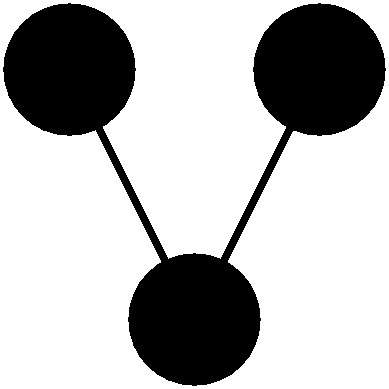
\epsfig{file = ../figures/Vmotif.eps, width=1cm, clip=} & 14\,113 & 25.5 & 514.9 & 3.36$\,10^{-1}$ \\
          \epsfig{file = ../figures/triangle.eps, width=1cm, clip=} & 75 & 10.4 & 6.2 & 2.87$\,10^{-1}$ \\
          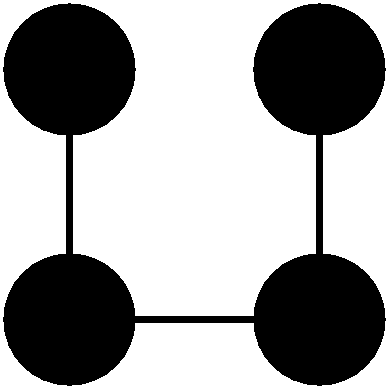
\epsfig{file = ../figures/chainmotif.eps, width=1cm, clip=} & 98\,697 & 11.9 & 7\,543.2 & 3.46$\,10^{-1}$ \\
          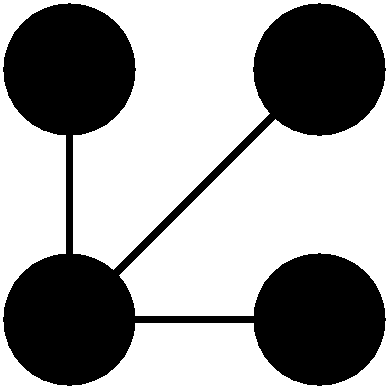
\epsfig{file = ../figures/starmotif.eps, width=1cm, clip=} & 112\,490 & 11.4 & 7\,812.0 & 1.85$\,10^{-1}$ \\
          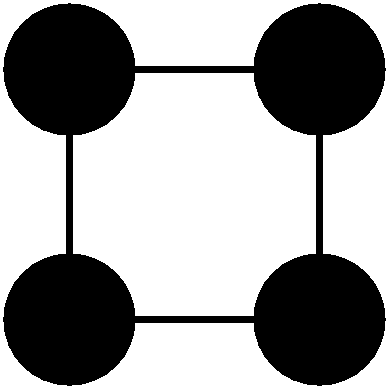
\epsfig{file = ../figures/squaremotif.eps, width=1cm, clip=} & 1\,058 & 5.9 & 82.9 & \emphase{9.34$\,10^{-3}$} \\
          \epsfig{file = ../figures/whisk.eps, width=1cm, clip=} & 3\,535 & 6.4 & 428.7 & 2.22$\,10^{-1}$ \\
          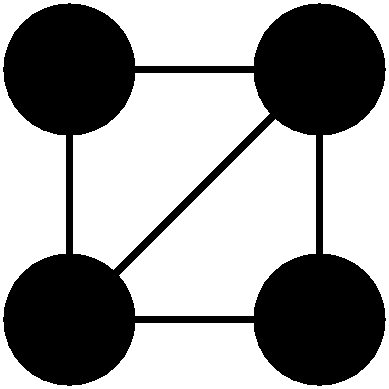
\epsfig{file = ../figures/halfclique.eps, width=1cm, clip=} & 79 & 2.9 & 11.5 & \emphase{2.56$\,10^{-2}$} \\
          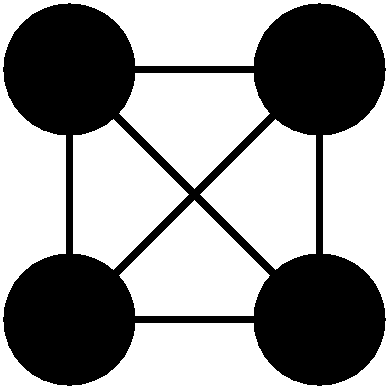
\epsfig{file = ../figures/clique.eps, width=1cm, clip=} & 0 & 0.1 & 1.1 & 1.00 \\
        \end{tabular}
        }
    \end{tabular}
  \end{tabular}

  {\bf Results for \emphase{E. coli}'s network.} 2 motifs
  appear to be unexpectedly frequent. \\
  ~\\
  According to the permutation-based strategy, all of them are
  significantly over-represented!
\end{frame}

%%%%%%%%%%%%%%%%%%%%%%%%%%%%%%%%%%%%%%%%%%%%%%%%%%%%%%%%%%%%%%%%%%%%%%%%
%%%%%%%%%%%%%%%%%%%%%%%%%%%%%%%%%%%%%%%%%%%%%%%%%%%%%%%%%%%%%%%%%%%%%%%%
\end{document}
%%%%%%%%%%%%%%%%%%%%%%%%%%%%%%%%%%%%%%%%%%%%%%%%%%%%%%%%%%%%%%%%%%%%%%%%
%%%%%%%%%%%%%%%%%%%%%%%%%%%%%%%%%%%%%%%%%%%%%%%%%%%%%%%%%%%%%%%%%%%%%%%%
